\section{Mathematical Formulation}
In this section, we establish certain mathematical notations that will be utilized to clarify the disagreement metrics.

\subsection{Saliency Maps}
For a given black box $b$ and a test instance $x$, where $x$ is an image of size $n \times n$, and an explanation method $c$, the saliency map explanation $e \in \mathbb{R}^{n\times n}$ for the black box $b$ with respect to test instance $x$ is obtained by running the attribution algorithm provided by $c$:
\begin{equation}
    e = c(b, x)
\end{equation}
Each value $e_{ij}$ represents the importance score that the pixel at $(i, j)$ contribute to the prediction of the black box $b$ at instance $x$. The range of values of $e_{ij}$ depends on the nature of the explanation method $c$.

\subsection{Metrics}
\label{subsec:metrics}
\subsubsection{Structural Similarity Index Metric}
To capture the similarity in structure between two saliency maps, we use the Structural Similarity Index Metric (SSIM) \cite{ssim}. Despite its name, this metric captures more than just structural similarity between two images: it takes into account the contrast, luminance, and the structure of two images.

For the sake of simplicity, given two saliency maps $e^{(1)}$ and $e^{(2)}$, let $x = e^{(1)}$, $y = e^{(2)}$. Then, the formula for SSIM between two saliency maps $x$ and $y$ is:
\begin{equation}
    \text{SSIM}(x, y) = [l(x, y)]^\alpha [c(x, y)]^\beta [s(x, y)]^\gamma
\end{equation}
where $l(x,y)$, $c(x,y)$, and $s(x,y)$ is the comparison of the luminance, contrast, and structure of two images $x$ and $y$, respectively; $\alpha$, $\beta$, and $\gamma$ are constansts that control the importance of the $l(x,y)$, $c(x,y)$, and $s(x,y)$, respectively.

Next, we present the definition of the three components of the SSIM. Let $\mu_x$, $\mu_y$ be the mean value of the saliency map $x$ and $y$; $\sigma_x$, $\sigma_y$ be the standard deviation of the $x$ and $y$; $\sigma_{xy}$ be the covariance of $x$ and $y$; $C_1$, $C_2$ and $C_3$ be small constants.

The luminance component is defined:
\begin{equation}
    l(x,y) = \frac{2\mu_x\mu_y + C_1}{\mu_x^2 + \mu_y^2 + C_1}
\end{equation}

Next, the contrast component is defined as:
\begin{equation}
    c(x,y) = \frac{2\sigma_x\sigma_y + C_2}{\sigma_x^2 + \sigma_y^2 + C_2}
\end{equation}

Finally, the structure component is defined as:
\begin{equation}
    s(x,y) = \frac{\sigma_{xy} + C_3}{\sigma_x\sigma_y + C_3}
\end{equation}

The constants $C_1$, $C_2$ and $C_3$ are typically set to small values in order to avoid zero division. $\alpha$, $\beta$ and $\gamma$ are usually set to 1, but they can be assigned with other values to emphasize or deemphasize their respective components.

In this work, because each saliency map differs in the range of its pixel values, we decided to measure SSIM using the magnitude of the saliency maps, normalized into the range $[0, 1]$ for fair comparison.

\subsubsection{Feature Agreement}
We utilize the feature agreement introduced by \cite{krishna_disagreement_problem}, adapted for images. For a saliency map $e$, a pixel $(i, j)$ is within the top-$k$ feature for $e$ if $|e_{ij}|$ is among the set of top-$k$ absolute values of all pixels of $e$. We denote the set of top-$k$ pixels of $e$ with $\text{top}_{k}(e)$. Then given two saliency map $e^{(1)}$ and $e^{(2)}$, the feature agreement between two maps is given by:

\begin{equation}
    \text{FA}_k(e^{(1)}, e^{(2)}) = \frac{|\text{top}_{k}(e^{(1)}) \cap \text{top}_{k}(e^{(2)})|}{k}
\end{equation}

Note that the above metric is equivalent to the following transformation and operation:
\begin{itemize}
    \item Taking the absolute value of both saliency maps
    \item Convert both saliency maps into a binary map in which pixels within top-$k$ are assigned the value 1, otherwise assigned the value 0
    \item The feature agreement of two saliency maps is computed by taking the size of the intersection of the 1s region and dividing by $k$
\end{itemize}

This metric captures how much the region that the two saliency maps consider most important overlaps with each other. Figure \ref{fig:featureAgreementDemo} presents the procedure to compute the feature agreement of a pair of explanations generated from Guided Backpropagation and Integrated Gradients. The feature agreement captures how much the two technique agrees for the top-5\% most salient pixels (for a $128\times128$ image, this is equivalent to $k= 820$).

\begin{figure}
    \centering
    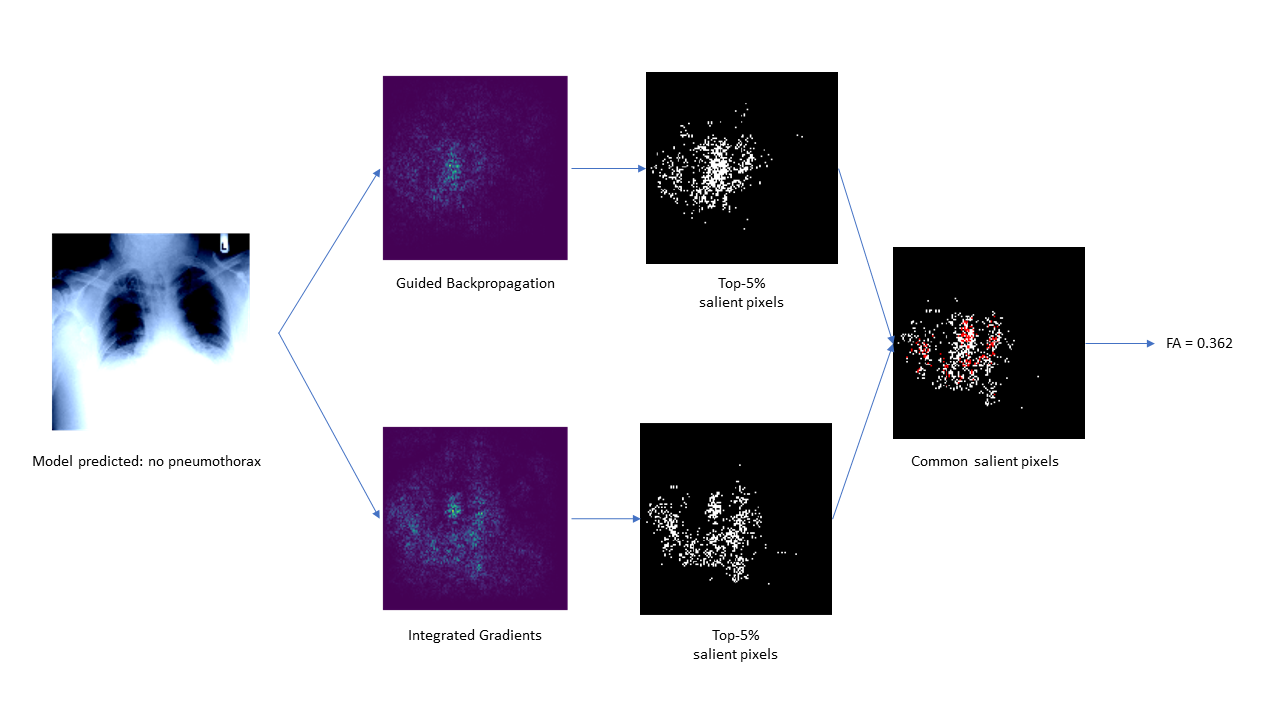
\includegraphics[width=\textwidth]{images/feature-agreement-demo.png}
    \caption{Illustration of how feature agreement was measured for an example pair of saliency maps generated by Guided Backpropagation and Integrated Gradients. We are interested in the top 5\% of the most important pixels ($k=820$ in total, colored white). The feature agreement score is calculated by determining the number of common top salient pixels (highlighted in red) and dividing this by $k$.}
    \label{fig:featureAgreementDemo}
\end{figure}


\subsubsection{Sign Agreement}
The sign agreement is quite similar to feature agreement, however, it is a stricter criterion \cite{krishna_disagreement_problem}. The sign agreement between two saliency maps $e^{(1)}$ and $e^{(2)}$ with respect to the top-$k$ features is:
\begin{equation}
    \text{SA}_k(e^{(1)}, e^{(2)}) = \frac{|\{(i, j) | (i, j) \in \text{top}_{k}(e^{(1)}) \cap \text{top}_{k}(e^{(2)}) \land e^{(1)}_{ij} \cdot e^{(2)}_{ij} > 0\}|}{k}
\end{equation}

The metric considers two saliency maps agree on a pixel if it is both significant in the two maps and has the same direction of contribution (negative or positive).

\subsubsection{Rank Correlation}
Another metric we adopted from the work of Krishna et al. \cite{krishna_disagreement_problem} is the rank correlation metric. In the original work, the metric is computed using the rankings of a subset of the input features. This feature subset when adapted to saliency maps can be represented as a mask. For any given matrix real matrix $d$ of size $m \times n$ (a saliency map can also be viewed as a matrix), a mask $m$ is a binary matrix of the same size, and the operation $m(d)$ return the set of $d_{ij}$ correspond to where $m_{ij} = 1$, that is:
\begin{equation}
    m(d) = \{d_{ij} | m_{ij} = 1, \forall i \in [1, m], \forall j \in [1, n]\}
\end{equation}

Given a saliency map $e$, we define $\text{rank}(e)$ to be the matrix of the rank of the pixel values of $e$. Then the rank correlation for two saliency maps $e^{(1)}$ and $e^{(2)}$ with respect to a mask $m$ is given by:
\begin{equation}
    \text{RC}(e^{(1)}, e^{(2)}, m) = r_s\left(m(\text{rank}(e^{(1)})), m(\text{rank}(e^{(2)}))\right)
\end{equation}